\documentclass[a4paper]{article}

%% Language and font encodings
\usepackage[english]{babel}
\usepackage[utf8x]{inputenc}
\usepackage[T1]{fontenc}

%% Sets page size and margins
\usepackage[a4paper,top=3cm,bottom=2cm,left=3cm,right=3cm,marginparwidth=1.75cm]{geometry}
\linespread{1.25}
%% Useful packages
\usepackage{amsmath}
\usepackage{graphicx}
\usepackage[colorinlistoftodos]{todonotes}
\usepackage[colorlinks=true, allcolors=blue]{hyperref}


\graphicspath{ {./figs} }

\begin{document} %{{{

\title{Novelty and Success of Fanfictions} %{{{
\date{\today}
\maketitle %}}}

\section{Introduction} %{{{
\label{sec:introduction}

It is widely believed that successful creative works strike a balance between novelty and familiarity. The classical inverted-U theory, also known as the Wundt-Berlyne curve, proposes that the perceiver's hedonic value first increases with novelty, until a certain threshold; afterwards, further increasing novelty will lead to a drop in hedonic value \cite{berlyne1970novelty}. Many experiments have been performed in seeking for empirical evidence for this theory \cite{hargreaves1984effects} \cite{sluckin1980liking}. However, it is still not clear where this assumed ``maximum novelty'' lies in the novelty -- familiarity continuum.

The contemporary popular culture has nurtured many creative works that are adaptations, remakes, and ``remixes" \cite{manovich2007comes} of previous works. In particular, the movies and TV industries have produced many stories that are variations of previously successful stories. For example, the stories of Sherlock Holmes has had more than 25,000 adaptations \cite{doyle2007new}. The DC Universe has ``rebooted" at least 3 times, and the Marvel Universe has more than 1,000 parallel universes \cite{marvelmultiverse}, each telling a slightly different story with the same set of characters. As an extreme example, the origin story of the Spider-man has been re-played in three movies since 2002 \cite{spiderman}. Market reception indicates that audience welcome this kind of stories: out of the 10 highest-grossing movies of 2016, 8 are sequels, remakes, or part of a movie universe \cite{2016film}.

This trend is also reflected in a new type of creative works --- fan works. Known formally as transformative works, they are creative works made by fans based on one or more original works (``canons''), and are often centered around certain characters or story lines\cite{wiki:transf_work}. For example, a story written by a contemporary fan about Sherlock Holmes in his retirement is considered a fan work. Although fan works contain multiple media types such as art, music and games, one of the most common type is creative writing---fanfictions. People interested in such activities often connect and interact with each other, forming communities known as fandoms\cite{wiki:fandom}. Fandoms have developed into very large communities, especially in the Internet. The data source of our study, ArchiveOfOurOwn.org, is an online fanfiction archive that allows users to upload their fictions, and categorizes them based on fandoms. Established in 2010, it has 1,313,000 users and 3,423,000 pieces of fanfictions by November 2017 \cite{ao3stats}.

Fanfictions as a unique cultural phenomena has drawn attention from media studies and cultural studies \cite{thomas2011fanfiction}. However, most of the studies focus on the identity of fanfiction writers\cite{black2006language}, the practice of fanfiction writing \cite{LIT:LIT12061}, and the interaction between fans \cite{hills2015expertise}. Relatively less studies have focused on fanfictions themselves as creative works, especially using quantitative methods\cite{zhaopredicting} \cite{yung2013market}.

The authors and readers' passion about fanfictions also alludes to a balance between novelty and familiarity: they desire to see familiar characters and elements, but in novel stories. By analyzing people's perception of fanfictions, we may gain a better understanding of this balance. The hedonic value of readers when reading fanfictions can be evaluated by how much they like a specific fanfiction:  In our dataset, the readers can click ``Kudos" (an equivalent of ``likes") if they enjoy reading a fiction, thus the number of Kudos can be used as a metric for hedonic value.

Researches are only starting towards a quantitative definition of novelty. Many have employed a networks research, defining a creative work's novelty by looking at how they reference previous works \cite{elgammal2015quantifying}\cite{wang2013quantifying}\cite{2017arXiv170704239I}. In some cases, tags of a work can be used to evaluate its novelty\cite{sreenivasan2013quantitative}. To quantify the novelty of fictions, we take an approach based on language modeling. Used widely in natural language processing and information retrieval\cite{jurafsky2000speech}\cite{Ponte:1998:LMA:290941.291008}, it represents documents as distributions over words. We can then compare documents by calculating the distance between these distributions. Thus we define novelty as ``the distance to average": more specifically, a fiction is more novel if it has a large distance from the average of previous fictions, and vice versa. Besides the language modeling approach, we also ran a separate analysis on the tag set of our fanfiction data. With our analysis, we show a negative relationship between novelty and success, indicating that fanfiction readers prefer more familiarity in general, discouraging novelty.


%Story telling is one of human beings' basic needs and abilities\cite{gottschall2012storytelling}. Despite having endless forms, most stories can be considered as variations of one of the basic archetypes. In mythology studies, Campbell deduced a fundamental structure, \emph{the hero's journey}, from all major myths around the world \cite{campbell2008hero}. Levi-Strauss broke down different versions of a myth to identify common mythemes \cite{levi1955structural}. In oral legends and tales, many stories had a certain origin and developed into different versions through time and interaction between creators. Myths and folktales in oral traditions of civilizations around the world often follow this pattern, for example, the tale of the \emph{Little Red Riding Hood} originated approximately in the 10th century, and has developed multiple variations\cite{littlered}. Some elements of the legend \emph{Mahabharata} can be traced back to the Vedic period (15--6 century B.C.) as oral tales told by bards, and was textualized into many versions\cite{van2011mahabharata}.

%Thomas \cite{thomas2011fanfiction} summarizes the study of fanfictions into several main stages: Earliest researches characterized the fanfiction writers as "rebels" against the powerful authority of the original work. Later researches attempted to generate a deeper understanding to this simplified view, and started responding to the new media forms that facilitated fan activities and interactions. Some recent studies shifted their emphasis to the contributions of fans to contemporary culture. 

% Similar to other creative works, fanfictions are constantly under selection and evaluation from their readers. %The most successful fanfictions in the market have been published and even adapted into other media forms, accepted by the main stream (for example, \emph{Fifty Shades of Grey} was originally a fanfiction of \emph{Twilight}), while the majority of them remain mostly unknown.





\section{Results} 
We first present some descriptive statistics of our data. Figure \ref{fig:fandom_size} shows the number of fictions in each of the 25 fandoms that we study. Figure  shows the time distribution of fictions. As AO3 was established in 2010, the fictions earlier than this time might be migrated from other platforms. 

\begin{figure}[htbp]
\begin{center}
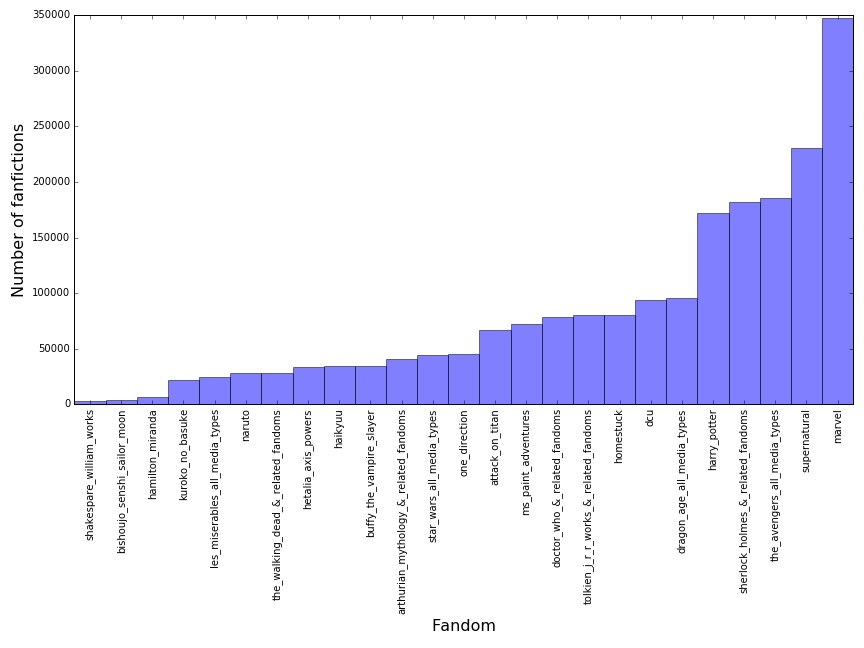
\includegraphics[width=0.7\textwidth]{/fandom_size.png}
\caption{Number of fanfictions in each fandom}
\label{fig:fandom_size}
\end{center}
\end{figure}


\label{sec:results}
\subsection{Novelty doesn't make fictions popular}
We define novelty as the cosine distance between a fiction and the typical fiction in its fandom. In the correlation matrix shown in figure \ref{fig:corr_heatmap}, we found that the cosine distance has a negative correlation with the hits/kudos that fictions receive. That is, the more creative a fiction is, the less kudos it will receive.

\begin{figure}[htbp]
\begin{center}
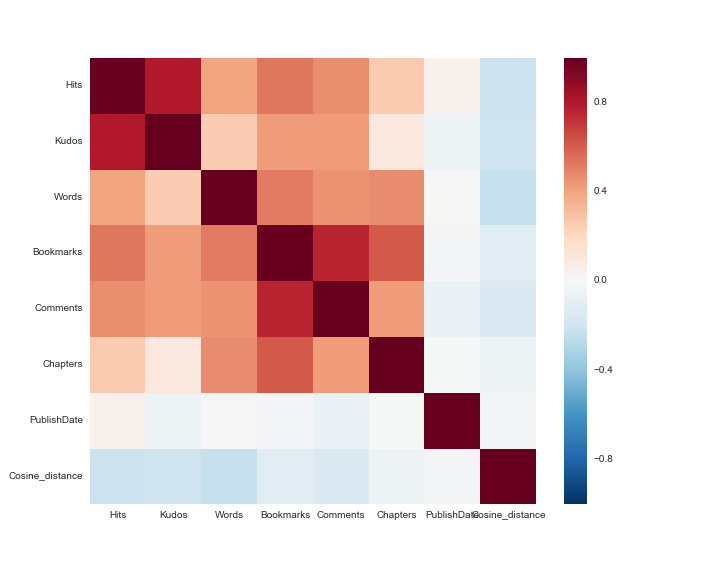
\includegraphics[width=0.8\textwidth]{/corr_heatmap_agg_1000.png}
\caption{Pairwise correlation between some important fields }
\label{fig:corr_heatmap}
\end{center}
\end{figure}

We further investigate this relation by fitting a negative binomial regression model. The result of the regression is summarized in figure \ref{regression_screenshot}. It can be observed that the cosine distance has a significant negative effect on Kudos.

\begin{figure}[htbp]
\begin{center}
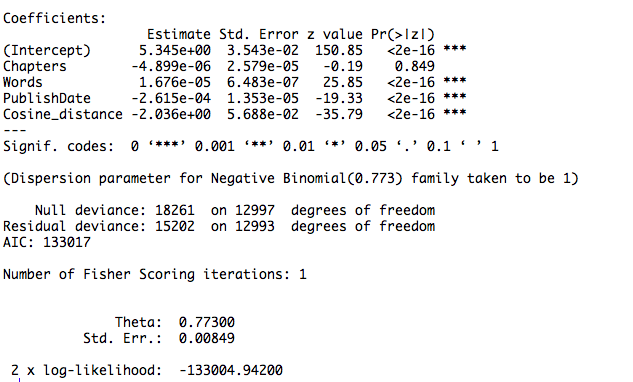
\includegraphics[width=0.8\textwidth]{/regression_screenshot.png}
\caption{Negative binomial regresion results}
\label{fig:regression}
\end{center}
\end{figure}

A closer look into cosine distance and Kudos is shown in figure \ref{fig:cos_kudos}. Because of the long-tailed distribution of Kudos, we choose to look at the log of Kudos. In general, the fandoms show the pattern that the average Kudos decrease when the cosine distance increases.


\begin{figure}[htbp]
\begin{center}
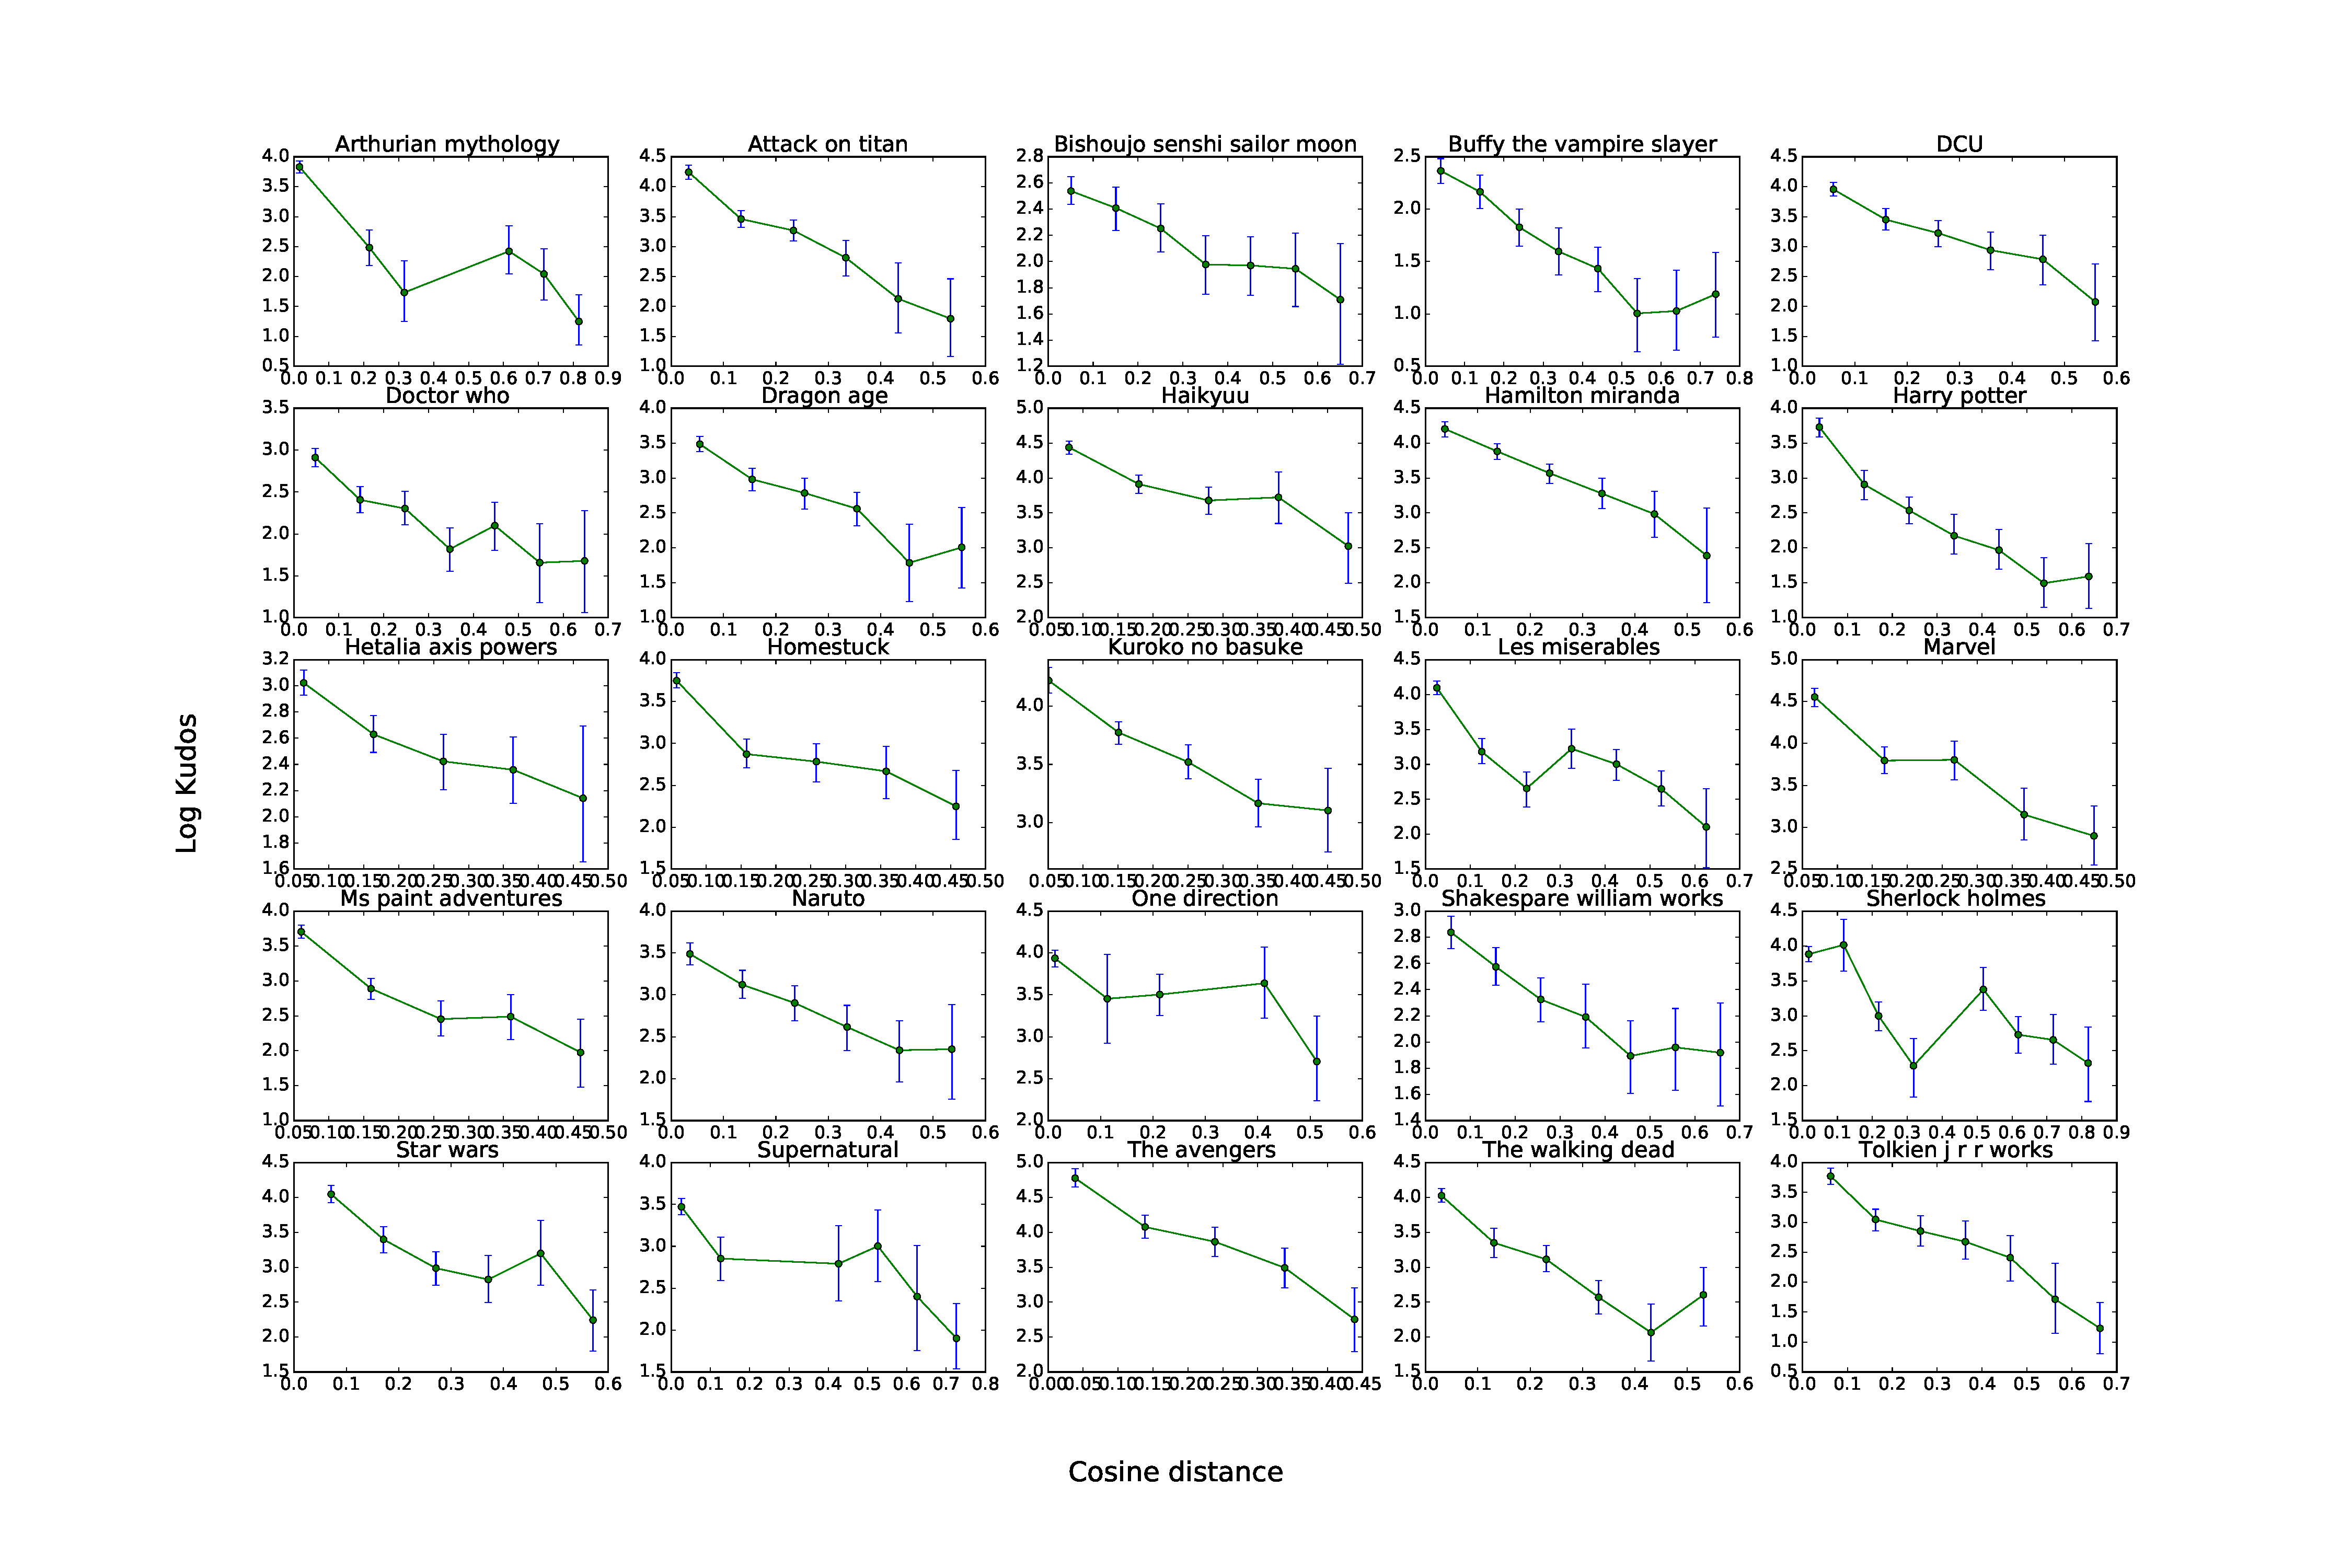
\includegraphics[width=\textwidth]{/cos_log_kudos_agg.pdf}
\caption{Cosine distance and the log of kudos.}
\label{fig:cos_kudos}
\end{center}
\end{figure}


%\subsection{The fandoms grow less creative?}


%}}}



\section{Methods} %{{{
\label{sec:methods}

%}}}

\subsection{Data}
We collected fanfictions from 50 fandoms according to AO3's list of most popular fandoms as of March 2016 \footnote{from this list: \url{http://archiveofourown.org/media}}. To avoid duplication, we remove fandoms with heavy overlapping (e.g.: we keep \emph{Marvel} and removed \emph{Marvel movies}). Fandoms that cover diverse topics (e.g.\emph{k-pop}) are also removed. Finally, we only kept the fictions written in English. This leaves us with 904,760 fictions from 25 fandoms. The number of fictions in each fandom is shown in .



Besides the work texts, we also collected metadata including 23 fields. We only used information contained in some of these fields. Table \ref{tab:metadata} gives the names and descriptions of these fields. 

\begin{table}[htp]
\caption{Metadata of the writings}
\begin{center}
\begin{tabular}[width=0.8\textwidth]{p{2cm}|p{4cm}|p{5cm}}
  \hline			
 Fields & Description & Usage\\ 
   \hline			
Text & The fiction texts. & All text analysis are carried out on these texts.\\\hline
Title & Titles of the fictions. & Used to identify the fictions. \\\hline
Fandoms & Describes which fandom(s) the fiction belongs to. & Used to categorize the fictions.\\\hline
Author & The author of the fiction. & Used for identifying the fictions and for text analysis. \\\hline
% Hits & The number of times a fiction is clicked on. & A metric for evaluating the fiction's popularity. \\\hline
Kudos & The number of times that readers "like" the fiction. &  A metric for evaluating the fiction's popularity.\\\hline
Publish Date & The date the fiction was published. & We use this to determine what time period a fiction belongs to. We also use the time between publish and now to evaluate the ``age" of a fiction.\\\hline
Chapters & The number of chapters that a fiction has. \\\hline
Words & The number of words in a fiction.\\\hline

\hline
\end{tabular}
\end{center}
\label{tab:metadata}
\end{table}%

Among the metadata fields, we're especially interested in the fields ``Hits" and ``Kudos", which shows how many times a fiction has been clicked or liked by readers. These are useful proxies for the popularity of a piece of work in a specific fandom.
Both statistics have power-law-like distribution, as shown in  Figure \ref{fig:long_tail}, proving our conception that the popularity of fictions is very imbalanced: most fictions are rarely read and receive little Kudos, while very few get the majority of views and Kudos.

\begin{figure}[htbp]
\begin{center}
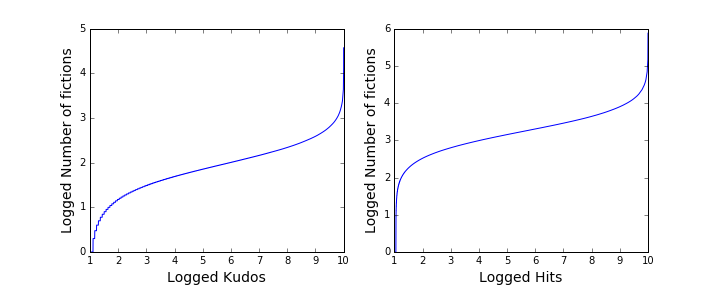
\includegraphics[width=\textwidth]{/kudos_hits_dist.png}
\caption{Log-log CCDF of the distribution of Kudos and Hits.}
\label{fig:long_tail}
\end{center}
\end{figure}

\subsection{Language model}
We model the fictions with a unigram language model. The Simple Good-Turing smoothing\cite{gales1995good} is applied to improve the model, and to assign non-zero probabilities to previously unseen unigrams. When creating the set of unigrams, we also remove the rare unigrams that appear in less than 5 documents and left out fictions with less than 500 words.

We verify that this model successfully captures the semantic and stylometrical contents of fictions. Using this model, the fictions from the same author are more close to each other compared to fictions from different authors, measuring by cosine distance, as shown in Figure \ref{fig:comparison_unigram_sgt}.

\begin{figure}[htbp]
\begin{center}
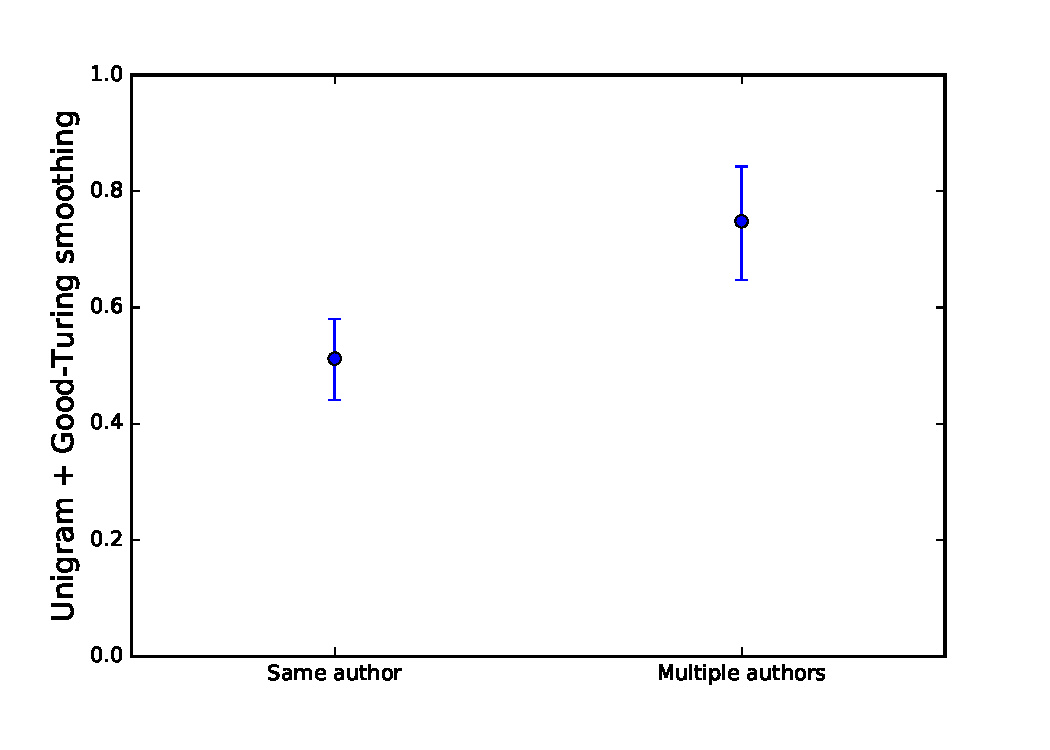
\includegraphics[width=0.6\textwidth]{/comparison_unigram_sgt.pdf}
\caption{Cosine distances between fictions from the same author and fictions from different authors in the Shakespeare fandom.
Left: The average cosine distance between fictions from same authors. In a 10-author dataset, average pairwise cosine distances between fictions from each author is calculated, and the overall distance is the average of the 10 groups. Right: The computation repeated on 10 random groups with the same size. The error bars are computed with the bootstrap resampling method. }
\label{fig:comparison_unigram_sgt}
\end{center}
\end{figure}

We further define the concept of a \emph{typical} fiction. A typical fiction of a fandom is the average of probability distributions of all fictions in the fandom. This allows us to calculate the distance between any fiction and the typical fiction. 

\subsection{Regression}
We apply a negative binomial regression using R's MASS library. 





\bibliographystyle{acm}
\bibliography{main}




    
\end{document} %}}}
